\documentclass[tikz]{standalone}

\definecolor{mplblue}{HTML}{1f77b4}

\tikzstyle{site}=[circle, minimum size=0.5cm, inner sep=0, fill=mplblue!20!white]

\begin{document}
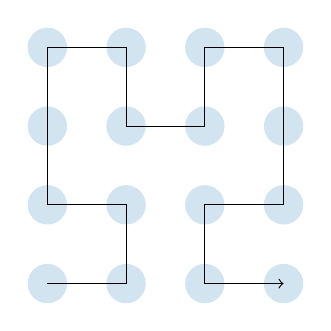
\begin{tikzpicture}

\node [site] at (0, 0) {};
\node [site] at (0, 1) {};
\node [site] at (0, 2) {};
\node [site] at (0, 3) {};
\node [site] at (1, 0) {};
\node [site] at (1, 1) {};
\node [site] at (1, 2) {};
\node [site] at (1, 3) {};
\node [site] at (2, 0) {};
\node [site] at (2, 1) {};
\node [site] at (2, 2) {};
\node [site] at (2, 3) {};
\node [site] at (3, 0) {};
\node [site] at (3, 1) {};
\node [site] at (3, 2) {};
\node [site] at (3, 3) {};

\draw [->] (0, 0) to (1, 0)
        to (1, 1) to (0, 1)
        to (0, 2) to (0, 3)
        to (1, 3) to (1, 2)
        to (2, 2) to (2, 3)
        to (3, 3) to (3, 2)
        to (3, 1) to (2, 1)
        to (2, 0) to (3, 0);

\end{tikzpicture}
\end{document}
